\documentclass{trlnotes}
\usepackage{trmath}
\addcompatiblelayout{thesis}
\setlayout{thesis}
\usepackage{trthm}
\usepackage{trsym} 
\usepackage{trphys}
\usepackage{silence}
% \usepackage{tikz}
\WarningFilter{latex}{Reference}
\graphicspath{{../../}}

\usepackage[
backend=biber,
sorting=none,
natbib=true,
style=authoryear,
language=russian
]{biblatex}
\addbibresource{../../thesisrefs.bib}
\begin{document}

Большая часть дисковых галактик во Вселенной содержат бар --- вытянутую морфологическую особенность, которая выделяется на 
фоне остальной галактики, если смотреть на неё в положении почти ``плашмя''. По данным современных инфракрасных 
обзоров, бары наблюдаются в 60\%-70\% галактик до красного смещения $z\sim 1$ \citep{marinova2007}.
В этом факте нет ничего неожиданного~"--- большая часть звёздных дисков в $N$-body моделях неустойчива
относительно образования бара, и необходимы специальные условия, чтобы подавить его формирование. В качестве такого фактора может выступать массивное тёмное гало или подсистема, обеспечивающая высокую
центральную концентрацию, например, сверхмассивная чёрная дыра \citep{shen2004} или компактный балдж
\citep{saha2018}. Более подробно о факторах, которые подавляют бароподобную неустойчивость, можно прочитать в статье \underdev \textcolor{red}{NS: сослаться на Селвуда}.

% \begin{figure}[htpb]
%   \centering
%   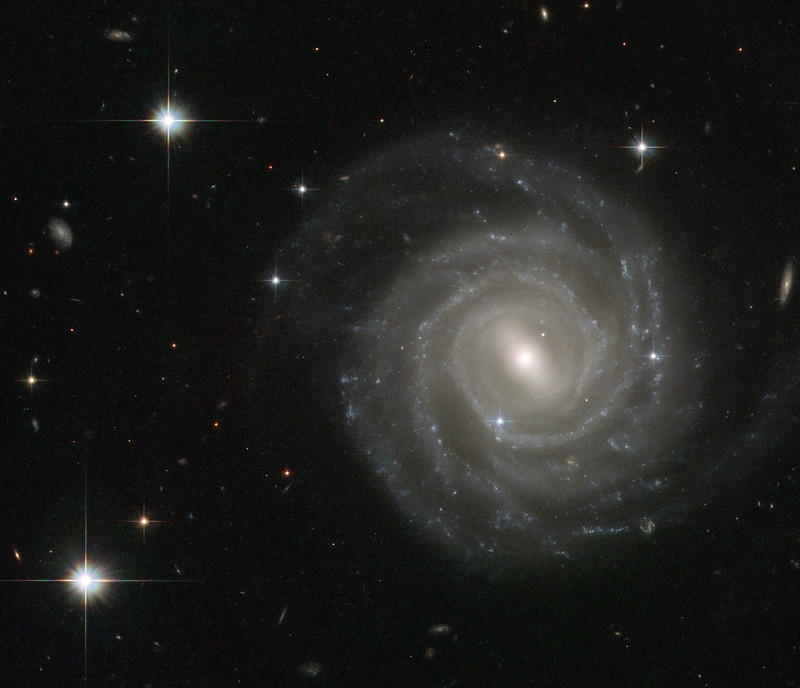
\includegraphics[width=0.8\linewidth]{img/intro/wp/ugc12158.jpg}
%   \caption{UGC 12158 --- галактика с выраженными спиральными рукавами и баром
%     \plholdev{а не барлинза ли тут, кстати}.
%     Пишут что она чем-то похожа на Млечный Путь, а снимок был снят чтобы запечатлеть
%     сверхновую SN 2004e.
%   Credit: ESA/Hubble \& NASA}%
%   \label{fig:frontpic}
% \end{figure}
%
% бессовестно скатано (не без неточностей) из обзора Атанасуллы в Secular evolution in disk galaxies
Как было показано в классических работах \citet{combes1981a} и \citet{raha1991}, вскоре после
образования бара в модельных расчётах, он <<выгибается>> из плоскости диска и на непродолжительное время теряет симметрию относительно неё. В
результате, галактика при взгляде с ребра показывает ящикообразную или арахисообразную форму, значительное
более утолщённую, чем бар на его начальных стадиях формирования. Подобные особенности наблюдались у реальных галактик задолго до их обнаружения в
модельных расчётах и, поскольку они  выступали за плоскость диска, то были названы B/PS (boxy/peanut-shaped) балджами. Например, в статье
\citet{burbidge1959} форма центральной области галактики NGC~128 описана как необычная, с наибольшей толщиной не в
центре диска, а в двух симметричных точках по обе стороны от центра\note{``...coming out of the nucleus itself like
a cross''!}, а в \citet{lutticke2000} из $\sim\!1350$ галактик, видимых с ребра, у $45\%$ были найдены B/PS балджи.
На основе многочисленных кинематических исследований была установлена прочная связь между B/PS балджами и внутренней, утолщённой в вертикальном направлении,  частью баров
\citep{kuijken1995,bureau1999,chung2004,bureau2006}. 

С точки зрения наблюдений,
наибольшую сложность представляет задача обнаружить бар в галактике, видимой с ребра. В частности, в приведённых выше статьях
было показано, что наличие бара приводит к характерной форме распределения лучевой скорости с двумя высокими пиками и образованию  <<восьмёрки>> на диаграмме $R - v_{\text{loc}}$. 
Подобная корреляция проявляется и при изучении фотометрических характеристик. \citet{lutticke2000a} изучали выборку 60 галактик с B/PS балджами. По форме
профилей яркости в разрезе вдоль большой оси и параллельно ей для 95\% рассмотренных галактик они  подтвердили наличие у галактик бара. 
К тому же, многие B/PS балджи вращаются цилиндрически, что в целом подтверждает их общую природу с баром. 
 
При взгляде на диск галактики в положении <<плашмя>> установить наличие или отсутствие в ней бара гораздо проще. Например, это можно сделать визуально или по изменению эллиптичности изофот. Однако, чтобы обнаружить в такой галактике B/PS балдж, необходима дополнительная информация, например, кинематические данные или металличность звёздного населения. В первом случае в качестве критерия наличия бара чаще всего используется профиль параметра
$h4$~"---  четвёртого члена в разложении в ряд Гаусса-Эрмита (\cite{vandermarel1993}) распределения лучевой
скорости вдоль большой оси бара. 
О существовании вертикальной арахисообразной структуры говорит наличие на таком профиле двух симметричных минимумов, обнаруженное как в $N$-body моделях \citep{debattista2005,iannuzzi2015}, так и в наблюдениях \citep{mendez-abreu2008}.

% не менее бессовестно перевел кусок Laurikainen & Salo в книжке Galactic bulges
Однако, не менее интересно понять, к каким отличиям в морфологии бара в положении  <<плашмя>> приводит наличие B/PS балджа. 
Инструментом для подобного исследования может выступать анализ изофот, основная идея которого заключается в поиске
отклонений формы изофот от эллипсов~"--- из $N$-body моделей вытекает, что для бара с B/PS балджем,
наблюдаемого на промежуточных углах наклона, изофоты имеют ящикообразную форму\note{не знаю на кого тут
сослаться --- \textcolor{red}{NS: например, Дебатиста 2016, 2017}}. Подобным образом с помощью NIR данных из обзора 2MASS  \citet{beaton2007} обнаружили B/PS структуру в галактике M~31 ($i = 77.5^\circ$). В работе \citet{erwin2013} были изучены 78 галактик с разными углами наклона с целью подбора оптимальных параметров для
одновременного обнаружения бара и B/PS балджа. При этом, авторы, после экстраполяции по выборке
подходящих галактик, пришли к выводу, что 2/3 баров должны проявляться с ребра как B/PS балджи, что в
целом согласуется с выводами \citet{lutticke2000a}, но не очень надёжно в силу небольшого размера выборки.

Для галактик, наблюдаемых под небольшими углами наклона, возможна и отличная от ящикообразной морфология бара.
Довольно часто наблюдаются линзовидные структуры, погруженные в бар в его центральной части. Подобная особенность
впервые широко обсуждалась в работе \citet{laurikainen2011} и была названа авторами \emph{барлинзой}.
Авторы статьи провели детальную классификацию $\sim\!200$ дисковых галактик ранних типов по данным наблюдений в
инфракрасном диапазоне, добавив условное обозначение для барлинз (bl) в ранее описанные в литературе типы
\citep{devaucouleurs1959,buta2010}). От центральных линз (nuclear lens) и обычных линз они отличаются
размером, который составляет около половины длины бара, а от классических балджей~"--- профилем плотности и кинематическими
характеристиками. 

Таким образом, бары по их морфологии в положении <<плашмя>> можно разделить на, как минимум, две выделяющиеся группы~"--- бары с
барлинзами и арахисообразные бары. Однако, статистические исследования числа баров разных типов представлены только в нескольких работах, и пока нет общепризнанного взгляда на этот вопрос. Например, \citet{li2017a} нашли, что при  небольших углах наклона ($0^\circ$ -- $40^\circ$) только $3\%$ процента баров от общего числа изученных объектов имеют арахисообразную форму, а $27\%$ демонстрируют морфологию барлинзы. А при больших углах наклона ($40^\circ$
-- $70^\circ$) эти доли составили $13\%$ и $12\%$,  соответственно. При этом доля галактик с барами вообще в обоих диапазонах отличается незначительно~"--- $74\%$ и $68\%$, так же как и доля галактик, бары в которых имеют
эллиптические изофоты (unbuckled в терминологии авторов). 

Природа барлинз и корреляция между числом баров разных типов на разных наклонениях не могли не вызывать интереса
исследователей в этой области. В статье \citet{athanassoula2013a} приводятся результаты $N$-body моделирования галактик с учетом газа и физических процессов 
в нём (звездообразование, высвечивание и т.п). В модельных галактиках на поздних стадиях эволюции  получилась вполне похожая на барлинзу структура (например, ~Fig.~4 оттуда). В работе  \citet{athanassoula2015} на основе сопоставимих размеров барлинз и B/PS балджей при фотометрической 
декомпозиции $N$-body моделей с учетом газодинамики делается вывод, что это проявления одной и той же структуры, 
видимой под разными углами наклона. В \cite{salo2017} авторы приходят к похожим выводам, анализируя, 
однако, результаты бесстолкновительных расчетов с классическим балджем, заданным в качестве начального условия, а не образующимся в результате звездообразования из  натекающего на центр галактики газа. 

Связь наблюдаемой морфологии бара с параметрами подстилающей галактики часто становится предметом исследований, в которых 
анализуются результаты $N$-body расчетов. Так, например,  \citet{athanassoula2002}  рассмотрели три модели: с массивным гало 
($M_h/M_d = 1.5$), с массивным диском ($M_h/M_d = 0.75$) и с массивным диском и массивным классическим балджем 
($M_h/M_d = 0.75$, $M_b/M_d = 0.6$). При этом, в первом случае образовывался мощный  бар, во втором случае наблюдалось скорее овалообразное искажение изофот, а в третьем~"--- что-то среднее между первым и вторым случаями. В уже упомянутой ранее 
статье \cite{salo2017}, авторы отмечают, что кривая вращения с большим градиентом скорости в центральной области, связанная с наличием компактого классического 
балджа или концентрированного темного гало, приводит к образованию бара с барлинзой, а более пологая кривая вращения --- при отсутствии балджа~"--- к арахисообразному бару. Важно отметить, что в последнем случае X-образные особенности проявляются даже при нулевом угле наклона (в положении <<плашмя>>).  
\citet{smirnov2018} подтвердили этот вывод и отметили, что варьирование других параметров модели, таких как 
параметр Тумре ($Q$) или начальная толщина диска ($Z_d$), могут приводить к возникновению барлинз в 
бесстолкновительных моделях даже при отсутствии балджа. Однако, параметры $Q$ или $Z_d$ (если галактика наблюдается <<плашмя>>) довольно сложно получить из наблюдательных 
данных, в отличие от массы и  эффективного радиуса балджа, которые определяются из  аккуратной фотометрической декомпозиции 
изображения галактики и анализа звездного населения. Например,  \citet{laurikainen2014}) для изученной ими выборки галактик нашли, что относительная масса балджа составляет 
$0.1$ полной массы светящегося вещества, вместо $0.35$, получающейся при неучете в фотометрической декомпозиции  барлинзы. Важно отметить, что и в наблюдениях
\citep{laurikainen2017}, и в моделях \citep{salo2017} возникает промежуточная ситуация~"--- на изображениях с барлинзами после применения к изображению процедуры нерезкого маскирования обнаруживаются X-образные детали (Fig~A.4, IC 1067 в первой статье). Причём это обнаруживается даже на депроецированных изображениях. Этот факт явно свидетельствуют о динамической природе морфологических различий. 

Анализ вертикальной структуры $N$-body моделей многокомпонентных галактик показывает связь параметров родительской
галактики с геометрическими параметрами B/PS структур \citep{smirnov2018}, а не только с морфологией бара
в положении <<плашмя>>. Подобная взаимосвязь основана на разнице в орбитальном составе B/PS балджей, образовавшихся в разных
потенциалах \citep{parul2020}. Вопрос об орбитах, поддерживающих трёхмерный бар, достаточно подробно освещён в
литературе (например в обзоре \cite{athanassoula2016}), однако, поскольку барлинзы были обнаружены относительно
недавно, их природа и орбитальный состав ещё во многом остаются неизвестными. Более того, нет ни одного исследования, целеноправленно поясвящённого этому вопросу.

Цель данной работы~"--- детальное изучение разницы в орбитальном составе баров с  различной морфологией. При этом будут исследованы бары, которые образуются в самосогласованных $N$-body расчётах, моделирующих эволюцию дисковых галактик. Важно подчеркнуть, что интересовать меня будут, в первую очередь, именно различия, возникающие при наблюдении модельных баров в положении <<плашмя>>, а вертикальная структура баров не будет основным вопросом дипломной работы. 

Основная структура работы следующая.

\begin{enumerate}
\item В главе~\ref{chap:model} описаны параметры $N$-body моделей, самосогласованная эволюция которых приводит к образованию как бара с барлинзой, так и
арахисообразного бара. Приводится схема методики проведения $N$-body моделирования.
\item В главе~\ref{chap:method} описан основной метод, который используется в работе~"--- анализ 
доминирующих частот.
\item Большая часть главы~\ref{chap:split} состоит в описании процедуры выделения орбитальных семейств~"---
близких по морфологии групп орбит, и в сравнении населённости разных орбитальных семейств для разных моделей. 
\item В главе~\ref{chap:orb} приведены основные орбиты для каждого из разобранных семейств.
\item И, наконец, в главе~\ref{chat:conc} суммируются полученные результаты и делаются основные выводы.
\end{enumerate}

\end{document}
% vim:wrapmargin=3
